%!TEX root = ../memoire.tex

\chapter{Implémentation et évaluation du système}\label{eval}

Au chapitre précédent, nous avions extraits des informations précieuses de VerbNet. Dans ce chapitre, nous expliquerons comment nous nous sommes servis des informations extraites en Python. Nous avons d'abord implémenter les dictionnaires dans GenDR. Puis nous nous sommes servis des structures générées pour plus rapidement construire les graphes sémantiques. Ceux-ci nous serviront à tester notre système. Cette section est séparée en trois parties. D'abord nous expliquons comment les dictionnaires sont architecturés mainantent. Puis nous expliquerons en quoi certaines règles de grammaire ont changé à l'aide d'un exemple retraçant la construction d'un arbre. Puis finalement, nous parlerons de l'évaluation en soi.

\section{Implémentation des verbes et de leurs patrons de régime: lexicon.dict et gpcon.dict}

Au chapitre \ref{chapgendr}, nous avons démontré comment l'information lexicale était encodée dans GenDR. Nous avions deux dictionnaires: semanticon et lexicon. Ici, nous en avons trois: semanticon, lexicon et gpcon. L'implémentation de VerbNet a donc eu pour effet la création d'un troisième dictionnaire et la modification du lexicon. Effectivement, l'architecture du semanticon est restée la même.

\subsection{Lexicon.dict 2.0}
Commençons par le lexicon. Anciennement le lexicon de GenDR était structuré ainsi: une diathèse triviale est encodée dans predicate, puis les classes verbales sont de trois types: verbes à 1 actant (sujet), verbe à un actant (transitif direct), verbe à un actant transitif indirect, verbe à deux actants ditransitif. Puis, en ce qui concerne les verbes, chaque verbe doit pointer vers un des types de verbes. Puis à l'intérieur du verbe, si un des actants syntaxiques a des contraintes particulières on l'encode là. Voir la figure \ref{lexicon}.

Dorénavant, le lexicon fonctionne ainsi:
attributs par défaut de toutes les classes: 
Verbes
Noms
Adjectifs
etc.

Voici à quoi les noms et verbes ressemblent.
\begin{lstlisting}[language=XML, caption = Attributs par défaut des classes]
// ================= VERBS =================

// VERB
// ----

verb {
  dpos = V
  spos = verb
}

// ================= NOUNS =================

// NOUN
// ----
// Common nouns.

noun {
  dpos = N
  spos = noun
  countable = yes
  gp = { id=NP dia=1}
}
\end{lstlisting}

Ensuite on liste tous les verbes (6393) qui pointent vers une classe verbale (de tout niveau de profondeur). Il s'agit de la partie qu'on a extrait à la figure \ref{extracmembre}.
Ça ressemble à cela

\begin{lstlisting}[language=XML, caption = Partie membre du lexicon]
/*
 =======================================================
                      VERBNET MEMBERS
 =======================================================
*/
open_5 : "spatial_configuration-47.6"
open_up : "establish-55.5-1"
operate : "other_cos-45.4"
oppose : "amalgamate-22.2-3"
ordain : "appoint-29.1"
order_1 : "get-13.5.1"
order_2 : "order-60-1"
organize_1 : "create-26.4"
organize_2 : "establish-55.5-1"
organize_3 : "force-59-1"
originate : "establish-55.5-1"
ornament_1 : "butter-9.9"
ornament_2 : "fill-9.8"
ornament_3 : "illustrate-25.3"
\end{lstlisting}

Montrer qu'on a pu le système des classes predicate, verb dt, verb dit, etc. Que maintenant on a juste verb pour la dpos et la spos. Le reste est encodé directement dans chaque classe verbale de VerbNet : diathèse, id des patrons (pas de fonctions lex.). Montrer comment les mécanismes d'héritage fonctionnent maintenant : members vers classe verbale et classe verbale vers 'verb' ou vers leurs classes mères pour hériter de leurs gps, etc. Montrer un exemple d'une lexie (parler de la désambiguisation) qui pointe vers une sous-classe donc qui hérite des trais de la classe et de leurs gps, etc. Expliquer comment nous avons contruit cette partie et comment ça fonctionne. ON réitère la diathèse à chaque gp, pas comme dans l'autre lexicon où une diathèse triviale est donnée à tous, et quand elle change, on l'explicite ponctuellement dans une entrée donnéequi en aurait besoin.

\begin{lstlisting}[language=XML, caption = Partie: Classes de VerbNet]
/*
=======================================================
                   VERBNET CLASSES
=======================================================
*/

"tell-37.2": verb {
  gp = { id=NP_V_NP  
	       dia=12 } // John informed me.
  gp = { id=NP_V_NP_PP_of_topic  
	       dia=123 } // John informed me of the situation. }
"tell-37.2-1": "tell-37.2" {
  gp = { id=NP_V_NP  
	       dia=12 } // Ellen told a story.
  gp = { id=NP_V_NP_PP_to_recipient 
		     dia=123 } // Ellen told a story to Helen.
  gp = { id=NP_V_NP_Dative_NP   
	       dia=132 } // Ellen told Helen a story. Ellen told me, 'Leave the room.'
  gp = { id=NP_V_NP
		     dia=13 } // Ellen told Helen.
  gp = { id=NP_V_NP_PP_about_topic
		     dia=132 } // Ellen told Helen about the situation.
}
\end{lstlisting}

Ensuite nous avons le reste du lexique: noms, adjectifs, adverbes, prépositions, déterminants,etc. Les entrées sont normalement vides, sauf lorsqu'elles font appel à une fonction lexicale. Nous n'avons encodé que l'usage des fonctions lexicales locatives de type: Locin, Locad, Locab. Elles fonctionnent lorsqu'une unité lexicale sélectionne la préposition à utiliser et non le verbe. C'est pourquoi elles sont encodées sous le nom qui la sélectionne. (j'en aurai parlé à la section précédente)

\begin{lstlisting}[language=XML, caption = Partie: Unités lexicales non-verbales]
/*
=======================================================
               NON-VERBAL LEXICAL ENTRIES     
=======================================================
*/
accountant : noun
acorn : noun
acquaitance  : noun
across : preposition
\end{lstlisting}

Maintenant que nous avons fini d'expliquer le nouveau lexicon. Passons au dictionnaire qui contient tous les propriétés syntaxiques des ID que nous avons vu à la figure X.

\subsection{gpcon.dict}
Le gpcon, un dictionnaire de patron de régime qui contient 278 identifiants de patrons de régime.
expliquer comment le lexicon fait appel au gpcon et pourquoi on l'a encodé ainsi. le id dans gp d'une entrée pointe vers une entrée de gp dans le gpcon. Celui-ci contient toutes les informations du patron de régime. Le fait de séparer les dictionnaires comme ça ressemble bcp aux méthodes vues par XTAG, FrameNet, FORGe,  etc. Les unités dans le gpcon sont les identifiants des GPS. Puis à l'intérieur on spécifie les propriétés syntaxiques. On spécifie le nombre d'actant syntaxique en jeu. L'union de ça et de la diathèse dans l'autre dictionnaire permet de rendre compte des phénomènes où 2 gps utilisent les mêmes actants, mais qu'en surface on les réalise dans des ordres différents avec des prépositions différentes ou sans prépositions. Donc l'ordre des actants syntaxiques est important puisque la diathèse se base là dessus. Puis les informations syntaxiques dans les actants sont utiles pour que le premier actant est contraint d'être un N par exemple, puis son deuxième un V. Puis de l'information de surface: la relation. Cela dicte au système comment appelé la relation entre le dépendant et son gouverneur. Cela fait en sorte que si on prend le premier GP \lstinline! NP_agent_V { I={rel=subjective dpos=N} }!, quand on utilise le patron de régime identifié comme Np agent V on veut que son premier actant syntaxique soit de type nominal et que sa réalisation de surface est une relation subjective. Nous avons aussi instauré un mécanisme pour tenir compte du fait que certains patrons de régime permettent deux prépositions qui compétitionnent pour le même actant syntaxique. c'est le cas quand on regarde le gp \lstinline!NP_asset_V_NP_PP_from_out_of! qui a dans son régime \lstinline!III={rel=oblique dpos=N prep=from}! et \lstinline!III={rel=oblique dpos=N prep="out of"}!. Ainsi, cela permet de paraphraser encore plus et nous pouvons tenir compte du fait que VerbNet avait spécifié cela. Finalement, en créant notre dictionnaire de patron de régime, nous nous sommes rendus compte qu'il existait énormément de doublons. Nous en avons un exemple dans cet extrait de dictionnaire. Np agent V et NP attribute V ont les mêmes propriété syntaxiques. Ce sont deux identifiants qui représentent la même chose. Ce scénario se répète souvent dans notre gpcon. C'est une conséquence de VerbNet qui considère qu'il s'agit de deux gps différents puisque les rôles thématiques sont utilisés dans VerbNet. Comme nous les remplaçons par des actants sémantiques puis syntaxiques, que ce soit un agent ou un attribut ne change pas grand chose. Comme nous voulions tester l'implémentation de VerbNet, nous n'avons pas pris le temps de remédier à cette situation, mais elle n'était pas encombrante. On pourrait prendre le temps de nettoyer le dictionnaire de patron de régime.

\begin{lstlisting}[language=XML, caption = Gpcon]
NP_agent_V {
   I={rel=subjective dpos=N}
}
NP_agent_V_NP {
   I={rel=subjective dpos=N}
   II={rel=dir_objective dpos=N}
}
NP_asset_V_NP_PP_from_out_of {
   I={rel=subjective dpos=N}
   II={rel=dir_objective dpos=N}
   III={rel=oblique dpos=N prep=from}
   III={rel=oblique dpos=N prep="out of"}
}
NP_attribute_V {
   I={rel=subjective dpos=N}
}
\end{lstlisting}

\section{Ajustement du module grammatical: un exemple}
Maitenant que nous avons montré à quoi les dictionnaires ressemblent, nous allons présenter un exemple servant à exemplifier comme les règles de grammaires et les dictionnaires interagissent. Cela nous permettra aussi de présenter les nouvelles règles et mécansimes utilisés pour l'implémentation de VerbNet.

\subsection{Input}
La phrase: The teacher talked about history to the students. Décrire un peu l'input

\begin{lstlisting}[language=XML, caption=Input textuel, label=text-input]
structure Sem S {
  S:1{
    talk_3:1{
      tense=PAST 
      1-> teacher:1
      2-> student:1
			3-> history:1
    }
    teacher:1{number=SG definiteness=DEF}
    history:1{number=SG definiteness=NO}
    student:1{number=PL definiteness=DEF}
    main-> talk_3:1
  }
}
\end{lstlisting}

L'input de la figure \ref{text-input} permet de générer 9 arbres de syntaxe profonde qui correspondent aux phrases suivantes : 1)The teacher talked, 2)The teacher talked to the students, 3)The teacher talked with the students, 4)the teacher talked to the students about history, 5)The teacher talked with the students about history, 6)the teacher talked, 7)the teacher talked about history to the students, 8)the teacher talked about history with the students, 9)the teacher talked about history.

Ces 9 arbres découlent des patrons de régime permis par le lexème \lex{talk\_3} qui pointe vers la classe "talk-37.5". Donc 9 structures profondes ont été réalisées à partir de cet input parce que tous les gp permettaient de prendre le graphe sémantique en entrée. L'input contenait 3 arguments: les actants sémantiques 1,2 et 3. Et tous les patrons de régime ici sont des combinaisons de ces 3 actants. D'ailleurs pour qu'un patron s'applique, il peut y avoir plus d'actants dans la structure sémantique, ça ne posera pas problème, car la manière qu'il choisi de réaliser le gp dépend de s'il est applicable ou non (expliquer avec gp selection). La raison pour laquelle les 9 gps ont été réalisés sera plus claire lorsque nous aurons passé au travers de l'exemple. Pour l'instant, nous allons prendre la strcuture syntaxique profonde qui aurait généré la phrase que nous souhaitons reproduire. Soit la 4e structure

\begin{lstlisting}[language=XML, caption=Input textuel de l'exemple]

"talk-37.5": verb {
  gp = { id=NP_V                           dia=1 } // Susan talked.
  gp = { id=NP_V_PP_to_co_agent            dia=12 } // Susan talked to Rachel.
  gp = { id=NP_V_PP_with_co_agent          dia=12 } // Susan talked with Rachel.
  gp = { id=NP_V_PP_to_co_agent_PP_about_topic dia=123 } // Susan talked to Rachel about the problem.
  gp = { id=NP_V_PP_with_co_agent_PP_about_topic dia=123 } // Susan talked with Rachel about the problem.
  gp = { id=NP_V                           dia=12 } // Susan and Rachel talked.
  gp = { id=NP_V_PP_about_topic_PP_to_co_agent dia=132 } // Susan talked about the problem to Rachel.
  gp = { id=NP_V_PP_about_topic_PP_with_co_agent dia=132 } // Susan talked about the problem with Rachel.
  gp = { id=NP_V_PP_about_topic            dia=13 } // Susan talked about the problems of modern America.
}
\end{lstlisting}

\subsection{Création et lexicalisation de la racine}:
D'abord, la première règle appliquée est la règle de racine (root\_standard). Elle crée la racine de l'arbre et impose une dpos=V et une finitude=FIN. Puis le noeud dominant en RSem est lexicalisé s'il satisfait les contraintes requises. La lexicalisation de talk\_3 est opérée grâce à la règle lex\_guess\_from\_lexicon. Nous en avions glissé un mot au chapitre \ref{chapgendr} lorsque nous parlions des règles de lexicalisation fallback qui permettent de déduire que le lexème talk\_3 qu'on retrouve dans le dictionnaire est probablement la correspondance du sens de \sem{talk\_3} qu'on aurait retrouvé dans le dictionnaire. D'ailleurs, c'est logique puisque talk\_2 et talk\_1 n'ont pas le même sens, donc on les sépare. Jusqu'à présent les deux premières règles sont identiques à GenDR comme nous l'avons vu à la section \ref{secexemple}.

\begin{figure}[htb]
	\centering
	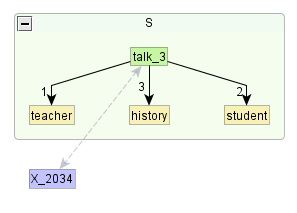
\includegraphics[width=0.5\textwidth, trim = {0cm 0cm 0cm 0cm},clip]{ch6/figs/root.png}
	\caption{Création de la racine à partir du noeud dominant}
	\label{deroulement0}
\end{figure}


\subsection{Sélection du patron de régime dans le lexicon}:
Ensuite, une fois que le noeud dominant est lexicalisé, la règle actant\_gp\_selection embarque. Ce qu'elle fait: elle prend le noeud (talk 3) puis elle regarde si cette entrée a un trait gp. Si oui, elle regarde dans le trait gp à la recherche de traits dia et id. ID est l'identifiant d'un patron de régime et dia fait en sorte que le gp sélectionnée se fasse en fonction de la disponibilité des actants sémantiques. Le trait dia nous dit aussi dans quel ordre les actants sémantiques se retrouvent en syntaxe.Il est essentiel qu'un lexème verbal aille chercher ces traits car il en a besoin pour appliquer les règles actancielles qui en découlent. Il faut que le système sache quel patron de régime utilisé pour un prédicat donné, et dans quel ordre les actants seront réalisés en syntaxe. La règle impose un gp au lexème en fonction de la diathèse du gp (quels actants sémantiques sont nécessaires à l'application du gp). Donc, de cette manière on s'assure que, après que la racine soit lexicalisée, seulement un gp traitant les actants sémantiques demandés en input sera utilisé. Dans le cas inverse, l'arborisation s'arrête brusquement après. Si la classe verbale contenait un gp dont la dia était 1234 ou bien 14, alors la réalisation n'aurait pas fonctionné, car il n'y a pas de quatrième actant dans la structure sémantique.

\begin{figure}[htb]
	\centering
	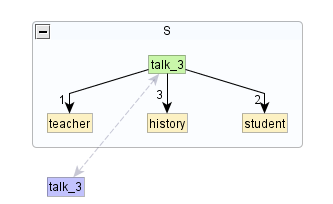
\includegraphics[width=1\textwidth, trim = {0cm 0cm 0cm 0cm},clip]{ch6/figs/selectiongp.png}
	\caption{Application de la règle actant\_gp\_selection}
	\label{deroulement1}
\end{figure}

\subsection{Règle actancielle: actant gp ijk}
Donc à l'étape précédente, le noeud lexical talk\_3 se fait imposer les restrictions suivantes: l'identification d'un gp et la diathèse qui vient avec. Cela va nous permettre d'appliquer cette règle. La règle actant gp ijk fait partie du groupe de règles actancielles que nous avons codés dans la grammaire. Dans GenDR, on regardait chaque arc individuellement, et on le faisait correspondre à une actant syntaxique dans le gp de l'entrée. Cela créait un arc entre la racine et un noeud vide mais contraints par les contraintes du gp. Maintenant ça ne fonctionne plus comme ça. Une fois que le gp est sélectionné, comme il a une diathèse de 3 actants sémantiques, il se fera imposer la règle qui réalise les relations actancielles à 3 actants (d'où le ijk). Nous en avons 6 pour réaliser des structures à 6 arguments. Dans notre cas, il fallait actant gp ijk.

La règle actant ijk, crée 3 arcs en partance talk\_3 au bout desquels se trouvent des noeuds vides sans contraintes. Les conditions pour que cette règle s'applique sont les suivantes: on veut que le noeud qui déclenche la règle soit lexicalisé, ait un patron de régime, et ait 3 actants sémantiques (les variables ijk). D'ailleurs, c'est à cette étape que le diathèse s'applique. Donc le passage des arcs sémantiques à syntaxique. Puisque la diathèse du gp X disait dia=123, cela se traduit par l'actant syntaxique I correspond au premier, puis ainsi de suite. Si on avait voulu que l'actant 2 soit l'actant syntaxique III, on aurait écrit la diathèse dia=132. Voir la figure \ref{deroulement2} \draft{en fait y'a un changement de diathèse, c'est pas la triviale, II devient 3 et III devient 2}

\begin{figure}[htb]
	\centering
	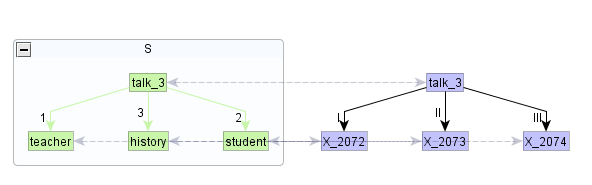
\includegraphics[width=1\textwidth, trim = {0cm 0cm 0cm 0cm},clip]{ch6/figs/actant_gp_ijk.png}
	\caption{Application d'une règle actancielle: actant\_gp\_ijk}
	\label{deroulement2}
\end{figure}

\subsection{Application des contraintes sur les noeuds}
Ensuite, il faut contraindre les noeuds créés lors de l'application de la règle précédente. Puisque avant les contraintes sur les noeuds se faisaient en utilisant le gp qui était dans le lexicon, on pouvait créer le noeud et le contraindre en même temps. Maintenant les restrictions sur les noeuds sont dans le gpcon, c'est pourquoi il faut une étape de plus. Donc cette règle dicte au système de regarder dans le gpcon pour le id du gp qui avait été sélectionné et contraindre les noeuds syntaxiques en fonctions des restrictions qu'ils ont (comme la dpos ou la finitude). La règle s'applique donc 3 fois puisqu'il y a trois noeuds vides. Voici les contraintes qu'on retrouve 

\subsection{lex standard}
Ensuite, on répète la règle de lexicalisation, puisque des noeuds vides n'attendent qu'à être lexicalisés s'il y a des lexèmes dans le lexicon qui peuvent satisfaire les contraintes des noeuds imposées à la règle précédente et qui correspondent à l'unité sémantique donnée en input. Dans cet exemple, c'est le cas et la règle lex\_standard s'applique donc 3 fois car il y a 3 noeuds à combler. Voir la figure \ref{deroulement3}

\begin{figure}[htb]
	\centering
	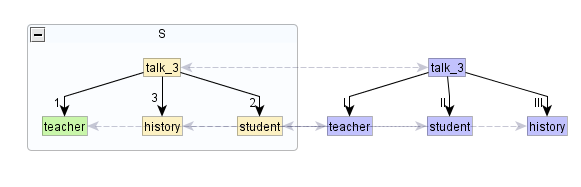
\includegraphics[width=1\textwidth, trim = {0cm 0cm 0cm 0cm},clip]{ch6/figs/lex.png}
	\caption{Application d'une règle de lexicalisation: lex\_standard}
	\label{deroulement3}
\end{figure}

\subsection{actant gp selection}

Finalement, la règle actant gp selection s'applique pour chaque noeud lexicalisé. Donc, à la fin, les lexèmes \lex{teacher},\lex{student} et \lex{history} ont leurs traits lexicaus en plus de l'identifiant d'un gp qui se trouve sous leur entrée et de la diathèse qui va de paire avec ce gp. Comme ce sont tous des noms communs, ils héritent du gp par défaut de la classe nominale id=NP dia=1 (nous n'avons pas plus d'information sur les patrons de régime des noms compte tenu que VerbNet se spécialisait dans les verbes, mais il existe d'autres ressources parmi celles que nous avions mentionnées qui pourrait combler cette lacune. c'est pourquoi nous n'avons que un gp pour les noms et qu'il est doté d'une diathèse simple permettant de faire la relation complément du nom). encore puisque ces nouveaux noeuds lexicalisés déclenchent l'application de la règle. Dès qu'un x a un gp, on va le repêcher, même si on s'en sert pas après. Dès qu'un noeud est lexicalisé, on regarde quel est son gp et on lui impose un gp. C'est pour cela qu'on se retrouve avec 9 réalisation profondes différentes. Parce que le verbe principal a 9 gps, sa lexicalisation a donc déclenché 9 occurrences de actant gp selection puisque le système scan pour tous les gps possibles et il créera un arbre différent à chaque fois.

Bref, grâce à toutes ces règles, nous avons opéré le passage de la RSem de x à la RSyntP de celle-ci. Une fois l'arborisation terminée, nous allons passé à structure syntaxique de surface.

\subsection{Lexicalisation des unités lexicales}
D'abord on applique une règle de lexicalisation de surface. Donc on va chercher deux traits: le lexicalisation de surface et la partie du disours de surface. Bref, c'est une simple règle de lexicalisation qui lexicalise les lexèmes à un niveau superficiel. Identique à ce qu'on a vu au chapitre 3.

\subsection{Règles actancielles de surface}
Une fois que les lexèmes sont réalisés en surface, les règles actancielles de surface se réalise. 3 règles actancielles seront appliquées puisqu'il y a 3 arcs de dépendances à réaliser. Cela fait en sorte qu'au lieu d'avoir l'étiquette des chiffres romains pour exprimer la dépendance syntaxique, on utilise le nom des relations. Donc, la règle synt\_subj est déclenchée et la relation subjective est belle et bien encodée dans le patron de régime de l'actant syntaxique I du patron de régime sélectionné \emph{NP\_V\_PP\_to\_co\_agent\_PP\_about\_topic}: \lstinline! I={rel=subjective dpos=N}!. Puis la règle actancielle de surface synt\_actant\_prep est déclenchée une première fois pour la relation syntaxique II entre talk et history, ce qui nous donne \lstinline! II={rel=oblique dpos=N prep=about}! que l'actant syntaxique II est identifiée par la relation oblique entre le dépendant et son gouverneur, puis il y a une préposition. Donc le noeud où était history se scinde en 2 pour que la préposition qui était encodées dans les traits de l'actant syntaxique soit réalisée en syntaxe de surface. Il s'agit d'un mot fonctionnel. Comme vous pouvez le voir dans la figure \ref{deroulement4}. Puis la règle synt\_actant\_prep est appliquée une seconde fois pour réaliser la relation syntaxique entre student et talk en syntaxe de surface. Encore une fois le noeud est scindé en deux pour laisser place à la préposition \lex{to} qui sera l'intermédiaire entre le verbe et l'actant syntaxique. La relation générée est objet indirect. Donc la seule différence entre l'application de ces règles entre la version qu'on a montré au chapitre GenDR et celle-ci, c'est le chemin que le système prend pour aller chercher ces informations. Il va dans le gpcon, trouve l'entrée gp qui correspond au trait ID sur le noeud principal et y cueille l'information.

\subsection{Règles des déterminants}
La règle det\_def réalise les déterminants qui doivent apparaître en syntaxe de surface. Ils correspondent aux traits que nous avions encodés dans l'input de départ. Seul \lex{teacher} et \lex{student} auront des déterminants puisque leur équivalent sémantique demandaient des définitudes qui s'était transmis jusqu'à la syntaxe profonde. Mais sont seulement réalisés en syntaxe de surface puisque ce sont des mots fonctionnels. La règle de déterminant réalise \lex{the} lorsque c'est défini et \lex{a} lorsque le noeud est marqué comme indéfini. C'est une règle propre à l'anglais.

\begin{figure}[htb]
	\centering
	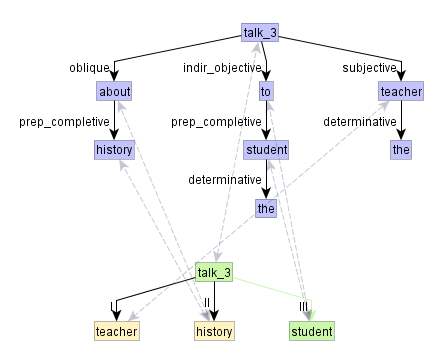
\includegraphics[width=1\textwidth, trim = {0cm 0cm 0cm 0cm},clip]{ch6/figs/ssynt.png}
	\caption{Applications des règles actancielles et réalisation des lexèmes fonctionnels}
	\label{deroulement4}
\end{figure}

Cela met fin à notre section implémentation. Nous avons démontré comment s'organisaient nos dictionnaires dorénavant et les nouvelles règles de grammaire qui ont tenu compte des changements apportés aux dictionnaires. Nous passerons donc à la phase évaluation pour voir comment a performé notre nouveau système.

\section{Évaluation}
Nous avons maintenant implémenté VerbNet dans GenDR. Nous sommes finalement rendu à l'étape d'évaluation du système. Cependant, avant d'entrer dans le vif du sujet, il serait pertinent de faire un bref retour sur les méthodes d'évaluation en \ac{GAT}. Il existe trois types classiques d'évaluation: basée sur l'application d'une tâche, humaine et automatique. \cite{ReiterBuildingNaturalLanguage2000} s'étaient déjà penché sur la question et pointaient en faveur d'une évaluation humaine. Toutefois, environ une décennie plus tard,  remarquaient que les méthodes d'évaluation automatiques se faisaient de plus en plus populaires. Notamment, la méthode BLEU qui avait été développée, à la base, pour les systèmes de traductions automatiques. Nous allons donc brièvement les décrire.

Les méthodes automatiques comme BLEU fonctionnent en comparant des outputs d'un système de traduction automatique à un ensemble de traductions humaine servant de point de référence. L'idée étant que la traduction automatique et la génération automatique comporte tous les deux l'aspect qu'un texte est produit par une machine en bout de ligne, et comme la méthode d'évaluation était appliquée au traduction automatique, plusieurs se sont dits qu'il serait intéressant de l'appliquerà la \ac{GAT} (Langkilde 2002; Habash 2004). Toutefois, certains réalisateurs mettent en garde contre la méthode BLEU. D'ailleurs, lors de son passage à SemEval, FORGe a aussi été évalué à la fois avec BLEU, et avec des évaluations humaines. Toutefois, FORGe mettent en garde que BLEU est bon pour évaluer la couverture mais pas nécessairement la qualité de chaque output (p.922-923). Leur système avait un score au dessus de la moyenne pour ce qui était de l'évaluation humaine. Mais un score plus faible pour la méthode BLEU et ce en raison de la couverture car FORGe avait mis de l'avant la qualité de ses outputs de sorte que son système filtre à deux reprises dans le pipeline des constructions fautives ou potentiellement fautives. C'est un cas classique de BLEU qui n'évalue pas toujours correctement des propriétés linguistiques cruciales (Scoot et Moore, 2007).

Les méthodes d'évaluation basées sur l'application d'une tâche sont assez courantes \citep{ReiterInvestigationValidityMetrics2009} et Belz semble dire qu'il s'agit de la méthode qui évalue le mieux le contenu des réalisations d'un système de \ac{GAT}. Toutefois elle nous met en garde que c'est la méthode la plus coûteuse en termes de temps et de ressources. En résumé, il s'agit d'évaluer les réalisations en utilisant le texte généré pour accomplir une tâche donnée. Plus l'output est lisible et clair, plus hautes sont les chances que la tâche soit réalisée rapidement et comme il le faut. Bref, la méthode la moins facile à mettre en place car il faut trouver des participants prêt à prendre de leur temps pour lire les rapports générés et effectuer une tâche. 

Finalement, il y a l'évaluation humaine, plus simple que la méthode à base de tâche, mais plus lente que la méthode automatique. Toutefois, cela reste une méthode très populaire dans le domaine. Il s'agit de coter les réalisations en fonction de leur performance à produire des phrases syntaxiquement et sémantiquement acceptables.

Considérant ces méthodes classiques, nous devons exclure en exclure deux: basée sur une tâche et automatique. D'abord notre système ne réalise pas du texte dans un but précis. On ne peut donc pas savoir si la phrase réalisée permettrait à un utilisateur d'accomplir une tâche en lisant le texte (et nous n'avons ni le temps, ni les ressources pour l'effectuer). Ensuite, nous ne pouvons pas utiliser la méthode automatique car notre système génère des arbres de dépendances de surface. Les systèmes utilisant la méthode automatique comparent des réalisations de surface où les textes sont linéarisées et morphologisés. Il est donc impossible pour nous de comparer nos arbres syntaxiques de surface avec du texte. Nous n'avons donc qu'une méthode d'évaluation devant nous: l'évaluation humaine basée sur des jugements.

\subsection{Mise en place de l'évaluation}
Pour procéder à l'évaluation de notre système, nous avons utilisé les outputs du script \ref{structurepython} au chapitre \ref{python} qui étaient des structures sémantiques vides.  Nous avons comblé les 978 structures vides en y encodant les unités et relations sémantiques qui correspondaient au sens de l'énoncé inscrit dans la structure vide. La tâche consiste à de donner ces structures sémantiques en input à notre système et évaluer le contenu qui en sortira.

Comme nous avions une quantité restreinte de temps, nous avons décidé de prendre un échantillon des 978 strucutres sémantiques. Nous avons choisi 75 structures sémantiques  aléatoirement. Parmi celles-ci, 25 ont servi à une partie développement précédent la phase d'évaluation comme telle. Ces 25 structures ont été passées au système afin de voir quels sont les problèmes immédiats que nous pouvons réglés sans vérifier comme tel si les arbres produits sont grammaticaux. Cette phase de développement nous a permi de constater qu'une bon nombre de nos inputs comportaient des problèmes. Si on ne règle pas ces problèmes, les réalisaitons échoueront nécessairement. La partie DEV nous a aussi permi de constater que certains lexèmes appartenant à des PDD différentes apparaissent en double dans notre dictionnaire. Par exemple le verbe \lex{work} et le nom \lex{work} ont la même forme. Cela a une incidence sur la réalisaiton puisque le système construit l'arbre syntaxique à partir du premier lexème qu'il rencontre. Donc si nous avions besoin du verbe dans l'arbre et que le système choisi le nom, alors nécessairement la réalisation échouera. C'est pourquoi nous avons procédé à un filtrage massif de ces cas et nous l'avons réglé en mettant une entrée sémantique dans le semanticon qui contient deux entrées lexicale. Une version verbale et une version nominale (on les distingue en mettant un \_n pour les noms.) ex : semanticon : work : lex=work lex=work\_n. C'est pas systématique de mettre le n après chaque nom,c'est seuelemnt quand y'a conflit de deux entrées identiques. La désambiguisation fait en sorte que class\_1 et class\_2 existent donc, dans notre exemple, nous n'avions pas à mettre class\_n dans l'entrée. Cela mit fin à la partie DEV.  Nous n'avons pas analysé en profondeur la nature des générations de ce niveau, nous voulions seulement corriger les problèmes de surface. Nous avons donc passé au peigne fin chacun des inputs de notre partie évaluation et nous nous sommes assurés que chaque unité lexicale n'avait qu'une seule forme dans notre dictionnaire. Des fois dans la structure y'a pas le bon verbe désambiguisé, il manque une relation, y'a une erreur de frappe, l'oubli d'un trait de définitude, etc.

Nous sommes ensuite passé à la phase d'évaluation comme telle en utilisant les 50 structure sémantiques restantes. Nous avons donc regardé chaque input de la partie EVAL pour nous assurer qu'ils soient en ordre, et nous avons scruté le lexique pour qu'il n'y ait pas de contradiction. Puis, nous avons entamé l'évaluation du système. Pour ce faire, nous avons développé un script qui prenait les structures d'input et les faisait passer à travers les permettant de visualiser les outputs de chaque input à tous les niveaux (RSem-RSyntP-RSynts). De plus, le script générait aussi une version textuelle (référence à GenDR) pour voir les traits des noeuds (partie du discours, finitude, id, dia, etc.) qui ne sont pas visibles dans le graphe visuel. 

\draft{demander à François comment on devrait calculer la précision. Est-ce que la réalisation de 9 arbres corrects pour 1 input est 9/9 ou 1/9 ? Parce que si on considère que c'est 1/9, alors on met les mauvaises réalisations et les réalisations grammaticales dans le même bateau.}
\FL{si pour un input tu produis 9 arbres et que ces 9 sont corrects, alors c'est 9/9. P=nb arbres corrects/nb arbres générés}
Nos critères étaient les suivants: le rappel et la précision. Pour notre expérience, le rappel s'évaluait de manière binaire. Si l'arbre syntaxique de surface correspond à la phrase que nous tentons de réaliser, alors la structure reçoit la note 1. Dans le cas contraire elle reçoit 0. Pour ce qui est de la précision, nous l'avons évalué comme suit. Pour le nombre d'outputs générés par structure, combien sont des arbres syntaxiquement et sémantiquement corrects représentant la phrase d'input (ou une partie de la phrase). Concrètement, pour le rappel nous évaluons le nombre total de 1 sur 50 (le nombre de structures testées). Puis, pour la précision, le nombre total de réalisations acceptables représentant la phrase (ou une partie de la phrase) sur le nombre de réalisations générées. Nous devons préciser une partie de la phrase puisque tous les patrons de régime d'une classe s'appliquent tel que nous l'avons vu dans l'exemple. Ainsi, un changement de diathèse donnera une réalistion acceptable, mais pas exactement la phrase qu'on veut représenter, et peut réaliser une partie de l'input sémantique comme dans 'the teacher talked about history' est une réalisation permise par l'input sémantique puisqu'il y a les actants nécessaires dans l'input et un patron permettant de réaliser cette phrase. Nous les avons compté parmi des réussites de précisions, car le but du système est de voir si l'implémentation de VerbNet dans GenDR s'est opérée correctement.
\FL{ta présentation du rappel et de la précision est inutilement compliquée. P=nb str correctes/nb str générées, R=nb str attendues qu'on peut générer/nb str attendues}

\subsection{Le rappel}

En ce qui concerne le rappel, nous avons un taux de 64\% brut. Toutefois, ce taux peut monter à 72\% si on omet les quelques erreurs d'encodage qui ont réussi à passer entre les mailles du filtrage que nous avions opéré précédemment. Ces erreurs d'encodage sont des détails qui n'aurait pris que quelques minutes à corriger. Ce qui a affecté le rappel est notamment causé par 5 problèmes. Ceux-ci sont de natures diverses: erreurs humaines, erreurs de VerbNet, problème d'incompatibilités théoriques, problème de MATE/GenDR.

Commeçons par les erreurs humaines. Celles-ci sont du même type que celles que nous avions repertoriés lors de la courte phase de développement. Nous en avons eu 4. Il s'agissait d'une erreur dans l'input où le verbe principal était grill\_3, mais il aurait fallu avoir grill\_1 pour avoir accès au bon patron de régime. Puis deux erreurs d'encodage de le lexicon et une erreur d'encodage dans le gpcon. Ce problème était inévitable puisque nous avons manuellement encodé 978 structures sémantiques. Ce qui a d'ailleurs agrandi le lexique.

Puis, les erreurs que nous avons importé directement de VerbNet. Ainsi, il y avait 2 cas où la structure sémantique demandait l'usage d'un verbe, mais ce verbe n'était pas répertorié par VerbNet. Donc comme ces verbes liaient des actants sémantiques, l'arborisation de ceux-ci n'a pas pu se faire correctement puisque GenDR n'avait pas accès aux patrons de régime de l'entrée. De plus, à quelques endroits, la structure sémantique de l'énoncé aurait demandé un patron de régime x, mais celui-ci ne figure parmi les patrons de régime répertorié par VerbNet pour cette entrée lexicale. Par exemple DO dans x want to do it. N'avions pas vu venir ce problème

Les erreurs humaines sont faciles à corriger. Dans un premier temps, nous corrigeons les inputs et les dictionnaires. Les erreurs de VerbNet pourraient être corrigées en allant chercher des patrons de régime de d'autres ressources pour compléter celles qui nous manque et pour aller chercher les entrées lexicales qui nous manque. Il s'agit d'erreurs relativement superficielles.

Les problèmes suivants sont de nature plus profondes. Parmi les structures qui ont failli au rappel, plusieurs le doive à problème d'interface sémantique-syntaxe de la part de VerbNet. À quelques reprises VerbNet considère qu'un patron de régime x est nécessaire pour représenter une énoncé, alors qu'en réalité, d'un point de vue sémantique, la représentation de la phrase et les patrons de régime fournis par VerbNet mèneront nécessairement à un échec de réalisation. Par exemple x and y verb. Ou bien x (verbe+cause) y.

\draft{Il existe d'autres problèmes similaires:  Ou bien, x laughed in embarasment ou bien x slept the sleep of the dead.Beaucoup de cas de verbe support. Donc, sémantiquement , si on se représente la phrase 'X took a flight' et qu'on considère que c'est took le verbe, sémantiquemet c'est faux. Take a flight est une collocation, dont le verbe support took n'est là que pour supporté le lexème flight. On pourrait paraphraser par flew. et on ne perdrait pas le sens. (montrer dans le semanticon comment c'est encoder et dans le lexicon) faire un bref retour sur les Oper. Devrait pas être dans le gp de take, mais plutôt dans les propriétés lexicales de flight, qui est sémantiquement fly. Donc dans GenDR, on peut traiter de ça. broke the window et the window broke. Le problème ici, c'est encore que ce sont deux sens de la même forme. briser et se briser. Cela fait en sorte que les gps partagés dans la classe ne devraient pas l'être. Voir les phrases avec slide aussi. Le même problème avec associated. on l'a au sens de x associe y à z et x s'associe à y.} Ce problème n'est pas surprenant, nous l'Avions vu venir lorsque nous créions les structures d'input.

Finalement, le dernier problème qui a grandement affecté le rappel est le mécanisme d'héritage de gp entre les classes dominées et les classes dominantes. Il s'agit du mécanisme dont nous vantions les mérites au début du chapitre. Concrètement, il s'agit d'un moyen qui fait en sorte qu'une class x pointe vers une classe y et hérite des traits encodés dans la classe y. C'est ainis que nous voulions implémanter l'architecture de VerbNet dans notre système. Mais il se trouve que le mécanisme d'héritage des traits fonctionne partiellement. Tel que présenté dans le début du chapitre, les unités lexicales pointent vers des classes verbales, une classe verbale peut pointer vers une autre classe verbale, et les classe verbales non-dominées pointent vers la classe verbe. Celle-ci donne les traits dpos=V et spos=verb à tous les lexèmes pointant vers des classes verbales. Ce mécanisme d'héritage foncitonne. Effectivement les unités lexicales réalisées ont tous les dpos et spos de la classe verbale, ce qui est un signe que le trait s'est propagé. Mais les patrons de régime ne semblent pas se transmettre d'une classe dominante à une classe dominée. Cela démontre donc que l'héritage des traits est partiel puisque les traits dpos et spos on transcendé toutes les classes subséquentes, mais les traits id et dia qui sont enfouis dans les traits gp (donc deux niveaux de profondeurs) n'ont pas fonctionné. Donc ce problème provient de MATE qui n'est pas capable de transmettre l'héritage d'un trait qui est enfoui dans un trait. Pour pallier à ce problème, on pourrait directement implémanter tous les gps des classes dominantes dans les classes dominées. Ainsi on garde l'architecture pensée de VerbNet où les classes héritent des patrons des autres classes. Le défaut de cette solution est que notre dictionnaire sera saturé d'information. Puisqu'il existe énormément de sous-classe. Cette solution est facilement adaptable puisque nous avons encore les scripts Python ayant servi à extraire les patrons de régime et à créer le lexicon. Nous n'avons qu'à modifier le script pour que chaque sous-classe hérite explicitement des gps des classe qui les domine. Évidemment, cela aura aussi un impact direct sur la précision, puisque dans notre expérience les verbes pointant vers une sous-classe x générait donc les gp de seulement les gp de la sous-classe. Si on fait ça, alors à chaque fois qu'on puise dans une sous-classe, tous les gps hérités feront aussi des tentatives de réalisation, ce qui alourdira le tout. Mais c'était ce qu'on avait prévu au début. Nous n'avions pas vu venir ce problème. Donner un exemple de ce problème. L'input x nécessite l'application du gp y pour la lexie z. La lexie z pointe vers une sous-classe w. Toutefois le gp y se trouve dans la classe mère et le système n'est pas capable d'aller le chercher puisque l'héritage des gps est deffectueux. Donc la réalisation de cet input devient impossile

\subsection{Précision}

En ce qui concerne la précision, nous avons un taux brut de (51\%).\FL{ouf, c'est bas! il faut distinguer entre les structures cul-de-sac et les vrais erreurs. ça te donne combien de P/R sur DEV?} Toutefois, si nous excluons les réalisations qui ne sont que l'application des deux premières règles (root et lex) 58\%. Le fait qu'une réalisation s'arrête brusquement après la racine est en quelque sorte une victoire du système puisque, le système a créé le noeud racine (systématique) puis l'a lexicalisé (systématique) et est aller chercher son gp avec gp selection (systématique) et la réalisation s'est arrêtée puisque le diathèse sélectionnée avec le gp ne correspondait pas aux actants sémantiques demandés par l'input. C'est un peu comme le système de FORGe qui estompe la réalisation lorsqu'il sait que ça me marchera pas. Finalement, en omettant les erreurs humaines d'encodage de notre part, ça nous amène à un taux de précision de 62\%.

\draft{Voici les pourcentages si on considère que la précision s'intreprète comme suit. Le calcul de l'arbre qu'on voulait générer /(sur) toutes les réalisations de surface (comprenant les réalisations grammaticales mais pas extacement correspondantes à l'input). Cela nous donnerait 23\%. Mais si on exclut la réalisation de la racine seule et les erreurs humaines, ça monte à 30\% .}

Ce qui a affecté la précision:
Mis à part la réalisation de la racine seule et des erreurs humaines, voici les phénomènes qui ont affecté la précision.

(si on considère les arbres partiels mais bons comme des erreurs de précision: Cela est dû aux patrons de régime le permettant et à notre module grammatical qui dit au système d'appliquer tous les patrons de régime possibles de la classe si la diathèse le permet. Exactement comme nous avons vu dans l'exemple au début où nous avions 9 réalisations de surface pour 1 input.)

Un cas classique qui est encodé dans plusieurs entrées de patron de régime est le cas où deux prépositions sont listées par VerbNet pour le même actant syntaxique. Par exemple, dans l'évaluation on a vu x. Et la sélection de la préposition y lors de la réalisation de surface rendait la phrase agrammaticale. quand deux prépositions compétitionnent pour le même actant syntaxique, le système génère les 2. C'est un problème qui nous est hérité de VerbNet et que nous n'avions pas prévu puisque nous pensions que VerbNet avait prévu des scénarios où deux prépositions compétitionnent pour la même place, mais qu'ils ne seront jamais parfaitement interchangeables. The doctor cured pat of pneumonia et the docteur cured pat out of pneumonia.

Une bonne partie du noise vient du fait que quand on réalise les gps, tous ceux d'une classe sont réalisés en surface. Le système prend le noeud dominant, il va cherhcher son équivalent dans le lexicon. celui-ci pointe vers une classe. Cette classe a des gps. Puis la règle sélection gp s'applique et pour chaque gp sélectionné, le système crée un nouvel arbre. Seuls ceux qui ont une diathèse qui correspond à la diathèse demandée en input seront réalisés encore plus loin et ceux qui ont un gp qui correspond à la diathèse d'une partie de l'input (teacher talked about history). C'est comme ça que notre système fonctionne et oui, ça créé du noise à chaque fois, mais on pourrait facilement s'en débarassé avec un filtre qui retire les constructions où on a seulement un noeud racine de l'arbre.

Toutefois, ce mécanisme cause du bruit quand un gp est sélectionné parce que les actants sémantiques demandées et ceux fournis par le gp sont un match. Là, il est possible qu'un gp soit utilisé et que ça mène à une réalisation de surface. Toutefois, il peut fort probablement y avoir une incompatibilité sémantique entre l'input et le gp, ce qui fait qu'il sera généré correctement en syntaxe, mais que la phrase est agrammaticale pour des raisons sémantiques ().

Ce mécanisme du à la manière que nos règles sont écrites affecte aussi le bruit en décuplant les arbres lorsqu'une structure d'input possède deux unités sémantiques qui se lexicalisent par des verbes. Effectivement le deuxième verbe pointe vers une classe verbale qui elle encode des patrons de régime, qui seront ensuite sélectionnés par la règle actant gp selection une fois que le noeud du deuxième verbe sera lexicalisé. Cela va donc créer des arbres différents jusqu'à ce que tous les ids des patrons de régime du deuxième verbe seront collés sur le noeud de l'arbre syntaxique profond. Cela génère donc des arbres différents à chaque fois. Exemple :quand on a deux verbes, puisque le système génère une réalisation différente pour chaque gp possible, même si I want to eat: on va avoir tous les gps possible de want , puis pour chaque gp de want permettant la réalisation de eat, on va aussi avoir tous les différents gp de eat qui vont se mettre sur le noeud eat, mais qui n'auront aucun impact sur la syntaxique puisque eat ne prend pas d'argument dans cette construction. Mais les noeuds réalisés sont différents donc ça génère un arbre de plus par gp de eat.

\subsection{Synthèse de l'évaluation}

Ce qu'on retire de tout cela sont deux problèmes majeurs. Le mécanisme d'héritage qui fonctionne partiellement avec l'architecture présente qui nuit au rappel et le mécanisme de sélection de patrons de régime post-lexicalisation qui nuit à la précision. Tel que nous l'avons mentionné, nous pouvons résoudre à court terme le problème d'héritage en implémentant les gps hérités directement dans les sous-classes. Toutefois, la solution à ce problème ne va qu'accentuer le second problème lié à la précision. Effectivement, en réglant le problème de cette façon, on augmente le nombre d'occurrence de l'application de la règle actant gp selection puisqu'elle devra s'appliquer pour tous les gps ajoutés dans la sous-classe.Toutefois, cela impliquerait un dictionnaire bcp plus lourd. Et cela impliquerait encore plus de noise. Ça augmenterait nettement le rappel, mais ça affecterait négativement la précision. À moins qu'on se dote d'un mécanisme pour filtrer les outputs.

De plus, il faut aussi tenir compte du fait que nous avons testé sur 5\% des structures d'input. Mais nous pensons que c'est un 5\% significatif car les problèmes mentionnés sont peu et ils apparaissaient plus d'une fois.

\draft{faire un retour sur l'évaluation en général, amener de nouvelles idées ?}
